\documentclass[conference]{IEEEtran}
\IEEEoverridecommandlockouts

\usepackage{cite}
\usepackage{amsmath,amssymb,amsfonts}
\usepackage{graphicx}
\usepackage{textcomp}
\usepackage{xcolor}
\usepackage{booktabs}
\usepackage{tabularx}
\usepackage{array}
\usepackage{multirow}
\usepackage{url}
\usepackage[hidelinks]{hyperref}

\graphicspath{{figures/}}
\newcommand{\sys}{\textsc{LicenseWise}}
\newcommand{\todo}[1]{{\color{magenta}\bfseries [To-do: #1]}}

\begin{document}

\title{LicenseWise: Explaining and Verifying Open-Source License Recommendations with LLMs and Natural Language Inference\\
{\large ENSF 621 --- Phase 2 Report}}

\author{\IEEEauthorblockN{Opeyemi Ajegbomogun}
\IEEEauthorblockA{\textit{Dept. of Electrical and Software Engineering} \\
\textit{University of Calgary}\\
Calgary, Canada}
\and
\IEEEauthorblockN{Okemawo Obadofin}
\IEEEauthorblockA{\textit{Dept. of Electrical and Software Engineering} \\
\textit{University of Calgary}\\
Calgary, Canada}
}

\maketitle

\begin{abstract}
Developers choose open-source licenses, or inherit them through dependencies, often without understanding the obligations involved. Large language models (LLMs) explain legal text fluently but also state unsupported facts, which is costly in licensing. \sys{} is a two-stage LLM\,+\,NLI system: an open-weight LLM recommends three licenses from a catalogue of 34 OSI-approved software licenses and explains each with plain-language claims that quote a specific clause, and an independent natural language inference (NLI) model marks every claim \emph{verified}, \emph{unverified}, or \emph{contradicted}. All ground truth is computed from public, curated license data, so no legal expert is needed. Phase~1 showed two weaknesses: the recommender broke stated requirements (top-pick accuracy 0.56), and the off-the-shelf verifier confirmed only 69\% of true claims. In Phase~2 we (1) grounded the recommender in the catalogue's license labels with a check-then-rank prompt, raising top-pick accuracy from 0.558 to 0.885 and top-3 accuracy from 0.740 to 0.942 on the same 104 descriptions, while a smaller model with the old prompt did slightly worse; (2) fine-tuned the top four layers of DeBERTa-v3-large on 729 clause--claim pairs, raising verifier accuracy from 0.815 to 0.925 and \emph{verified} precision from 0.944 to 0.978 on 146 human-labelled pairs (0.911 and 0.933 when the claim wording is unseen); and (3) turned the prototype into a connected web application with a FastAPI backend, a SQLite job store, a 27-test suite, and GitHub Actions CI on a two-branch workflow. Requests for weak copyleft remain the main failure case.
\end{abstract}

\begin{IEEEkeywords}
open-source licensing, large language models, natural language inference, explainability, fine-tuning, software engineering for ML
\end{IEEEkeywords}

\section{Introduction}
\label{s:intro}

\subsection{Problem}
Every piece of shared software carries a license that governs how others may use, modify, and redistribute it, and every dependency brings its own terms. Developers make these decisions with little legal training and often misunderstand obligations such as copyleft or patent grants~\cite{almeida2017developers,wu2024license}. Two failures follow: a \emph{wrong fit}, where the license does not protect what the developer cares about (e.g., a permissive license when improvements were meant to stay open), and a \emph{conflict} with a dependency's license (e.g., proprietary terms on top of a strong-copyleft component). Existing help does not fit the individual project. Decision guides such as choosealicense.com~\cite{choosealicense} offer a few generic paths and ignore dependencies; scanners and compliance tools~\cite{german2010ninka,scancode,xu2023lidetector} audit code after it is written; lawyers are accurate but slow and costly for students and small teams. LLM chatbots explain licenses well but produce confident statements the source text does not support~\cite{ji2023hallucination,maynez2020faithfulness}, and in licensing a confident wrong answer is worse than none.

\subsection{Solution and Innovation}
\sys{} recommends a license for a specific project \emph{before} code is released and makes its explanation checkable. Three ideas distinguish it: (1) the LLM recommends and explains only from a curated catalogue, and each claim must cite and quote one license clause; (2) an independent NLI verifier, adapted to license language by fine-tuning in Phase~2, labels each claim against its clause, and the user can open the clause in one click; and (3) the evaluation is \emph{expert-free}: answer keys are computed from public license labels rather than judged by opinion. Licensing is one of the first decisions in every open-source project, so a project-specific, checkable answer lowers legal risk for exactly the users who cannot afford a lawyer.

\subsection{Research Questions}
Phase~2 refines the Phase~1 questions; the additions are in italics.
\begin{itemize}
    \item \textbf{RQ1 (requirement-to-license mapping).} To what extent can an open-weight LLM, conditioned on a curated license catalogue, map natural-language project requirements to licenses that satisfy them; how does accuracy vary with requirement specificity; \emph{and how much does grounding the model in the catalogue's license labels help?}
    \item \textbf{RQ2 (claim verification).} How reliably can NLI models, \emph{off the shelf and adapted to license text by fine-tuning}, verify LLM-generated claims against the clauses they cite, measured on human-validated clause--claim pairs?
    \item \textbf{RQ3 (explanation faithfulness).} To what extent are LLM-generated explanations grounded in the cited text (quote fidelity, entailment), and how does NLI verification change the claims shown to developers compared with an unverified baseline?
\end{itemize}

Table~\ref{tab:shaw} classifies the questions with Shaw's scheme for software engineering research~\cite{shaw2003writing}.

\begin{table}[tb]
    \caption{Research questions in Shaw's categories~\cite{shaw2003writing}.}
    \label{tab:shaw}
    \centering
    \footnotesize
    \begin{tabularx}{\columnwidth}{@{}l>{\raggedright\arraybackslash}X>{\raggedright\arraybackslash}X>{\raggedright\arraybackslash}X@{}}
        \toprule
        & \textbf{Question type} & \textbf{Result type} & \textbf{Validation} \\
        \midrule
        RQ1 & Method of development & Procedure (prompt v1 $\rightarrow$ v2) & Analysis: paired experiment, 104 descriptions, computed keys \\
        RQ2 & Method for analysis & Technique + empirical model (fine-tuned verifier) & Analysis: grouped cross-validation, human-labelled test set \\
        RQ3 & Characterisation of a system & Specific solution (verified pipeline) & Evaluation: verified vs.\ unverified claims on real runs \\
        \bottomrule
    \end{tabularx}
\end{table}

\subsection{Contributions of Phase 2}
\begin{itemize}
    \item A \textbf{connected application}: React UI, FastAPI backend with asynchronous jobs, SQLite history, tests, and CI/CD on a two-branch GitHub workflow (Section~\ref{s:system}).
    \item A \textbf{label-grounded recommender} (prompt v2) and a model-size comparison, evaluated on the same 104 descriptions as Phase~1 (Sections~\ref{ss:stage1method} and~\ref{ss:rq1}).
    \item A \textbf{fine-tuned license verifier} trained on a laptop by caching frozen layers, with a test of whether it memorises claim wording (Sections~\ref{ss:verifiermethod} and~\ref{ss:rq2}).
\end{itemize}

\section{Related Work}
\label{s:related}

\subsubsection{Understanding and identifying licenses}
Developers misunderstand license terms and combinations~\cite{almeida2017developers}, and license use in practice is complex and error-prone~\cite{wu2024license}. Ninka~\cite{german2010ninka} and ScanCode~\cite{scancode} identify licenses in files, machine learning detects license exceptions~\cite{vendome2017exceptions}, and LtRecognizer recognises license terms with NLP and LLMs~\cite{liu2027ltrecognizer}. These works \emph{identify} what is present; \sys{} \emph{recommends} and explains.

\subsubsection{Compatibility and compliance}
Kapitsaki et al.\ check compatibility from SPDX metadata~\cite{kapitsaki2017spdx}, LiDetector finds incompatibilities in a project~\cite{xu2023lidetector}, and the OSADL matrix~\cite{osadl} encodes which licenses combine. They audit existing code and do not explain their verdicts.

\subsubsection{License data}
The SPDX list~\cite{spdx} standardises identifiers, choosealicense.com~\cite{choosealicense} publishes machine-readable permission, condition, and limitation labels, and the Software Heritage archive~\cite{dicosmo2017swh} underlies a dataset of 6.5 million license files~\cite{zacchiroli2022dataset}. We use all three.

\subsubsection{Faithfulness and NLI verification}
Hallucination is a known weakness of neural generation~\cite{ji2023hallucination,maynez2020faithfulness}. NLI models trained on MNLI~\cite{williams2018mnli} and ANLI~\cite{nie2020anli} detect inconsistencies between a source and generated text~\cite{laban2022summac,honovich2022true}, and retrieval-augmented generation grounds outputs in retrieved passages~\cite{lewis2020rag}. Grounding alone does not produce a per-claim verdict; \sys{} combines quoting a retrieved clause with an NLI check by DeBERTa-v3~\cite{he2023debertav3}.

\subsubsection{The gap}
No existing tool both recommends a license for a specific project before release and verifies its own plain-language explanation against the license text.

\section{Overview of Phase 1}
\label{s:phase1}

\subsubsection{Pipeline}
Given a project description and/or a dependency manifest, the Phase~1 pipeline (i) looks up each dependency's declared license on PyPI or npm and normalises it to SPDX; (ii) Stage~1: gpt-oss-120b, an open-weight LLM served by Groq~\cite{groq}, recommends exactly three licenses from the catalogue, with JSON-schema-constrained output; (iii) retrieves the clauses that express each license's obligations; (iv) Stage~2: the LLM writes three to five claims per license, each citing one clause and quoting it verbatim; and (v) checks every quote and runs DeBERTa-v3-large NLI~\cite{he2023debertav3,laurer2024less} with the clause as premise and the claim as hypothesis. A command-line interface and a React UI that displayed saved results were built.

\subsubsection{Data, built without a legal expert}
From choosealicense.com and SPDX we kept the \textbf{34} OSI-approved software licenses and split them into 812 clauses. For RQ1, six requirements a developer would state (copyleft level, network use, patent grant, trademark, attribution, change documentation) give 191 requirement combinations; computing which licenses satisfy each from the labels leaves \textbf{77 profiles} with known answer keys. One LLM (Qwen) wrote first-person project descriptions from the profiles, and a different LLM (gpt-oss-20b) checked them blind; \textbf{190} passed. For RQ2, templates produced \textbf{729 clause--claim pairs} (entailment, neutral, contradiction); two annotators checked \textbf{146} of them, agreeing with the automatic labels on 97.9\% (Cohen's $\kappa = 0.88$~\cite{cohen1960kappa}).

\subsubsection{Results and open issues}
On 104 descriptions covering all 70 described profiles, Stage~1 reached Hit@1 0.56 and Hit@3 0.74, but Hit@3 fell to 0.60 when only one to three licenses fit. Picks often broke stated requirements: trademark protection (54\% of picks), no obligation to document changes (39\%), copyleft level (21\%). DeBERTa outperformed RoBERTa-large-MNLI (accuracy 0.815 vs.\ 0.733) and was reliable when it said \emph{verified} (precision 0.944), but confirmed only 69\% of true claims. In two end-to-end runs all 19 quotes were verbatim and 58\% of claims were verified. The UI was not connected to a backend. These issues defined Phase~2.

\section{Software Solution}
\label{s:system}

\subsection{Architecture Evolution}
\label{ss:arch}

Figure~\ref{fig:arch} shows the Phase~2 architecture. The Phase~1 design already planned a web UI calling a FastAPI backend that runs the pipeline; Phase~2 built it. Four things changed relative to the Phase~1 plan. (1) The REST interface became a single resource, \texttt{/api/recommendations}, created with \texttt{POST} and polled with \texttt{GET}, instead of separate \texttt{/recommend} and \texttt{/jobs/\{id\}} endpoints. (2) Jobs are stored in SQLite instead of an in-memory cache. (3) Stage~1 uses prompt v2 (Section~\ref{ss:stage1method}). (4) The verifier is fine-tuned (Section~\ref{ss:verifiermethod}). Two planned components were \emph{not} built and remain future work: a rule engine with the OSADL compatibility matrix, and vector retrieval, which is still replaced by deterministic clause selection because full license texts exceed the free tier's per-minute token limit.

A run takes 30\,s to 5\,min on the free tier, too long for one HTTP request. \texttt{POST} therefore validates the input and returns \texttt{202} with a job identifier at once; one worker thread runs jobs in order, because Groq's per-minute limit and the single verifier in memory make parallel runs slower, not faster. The UI polls every 1.5\,s and shows the current step and queue position.

\begin{figure*}[tb]
    \centering
    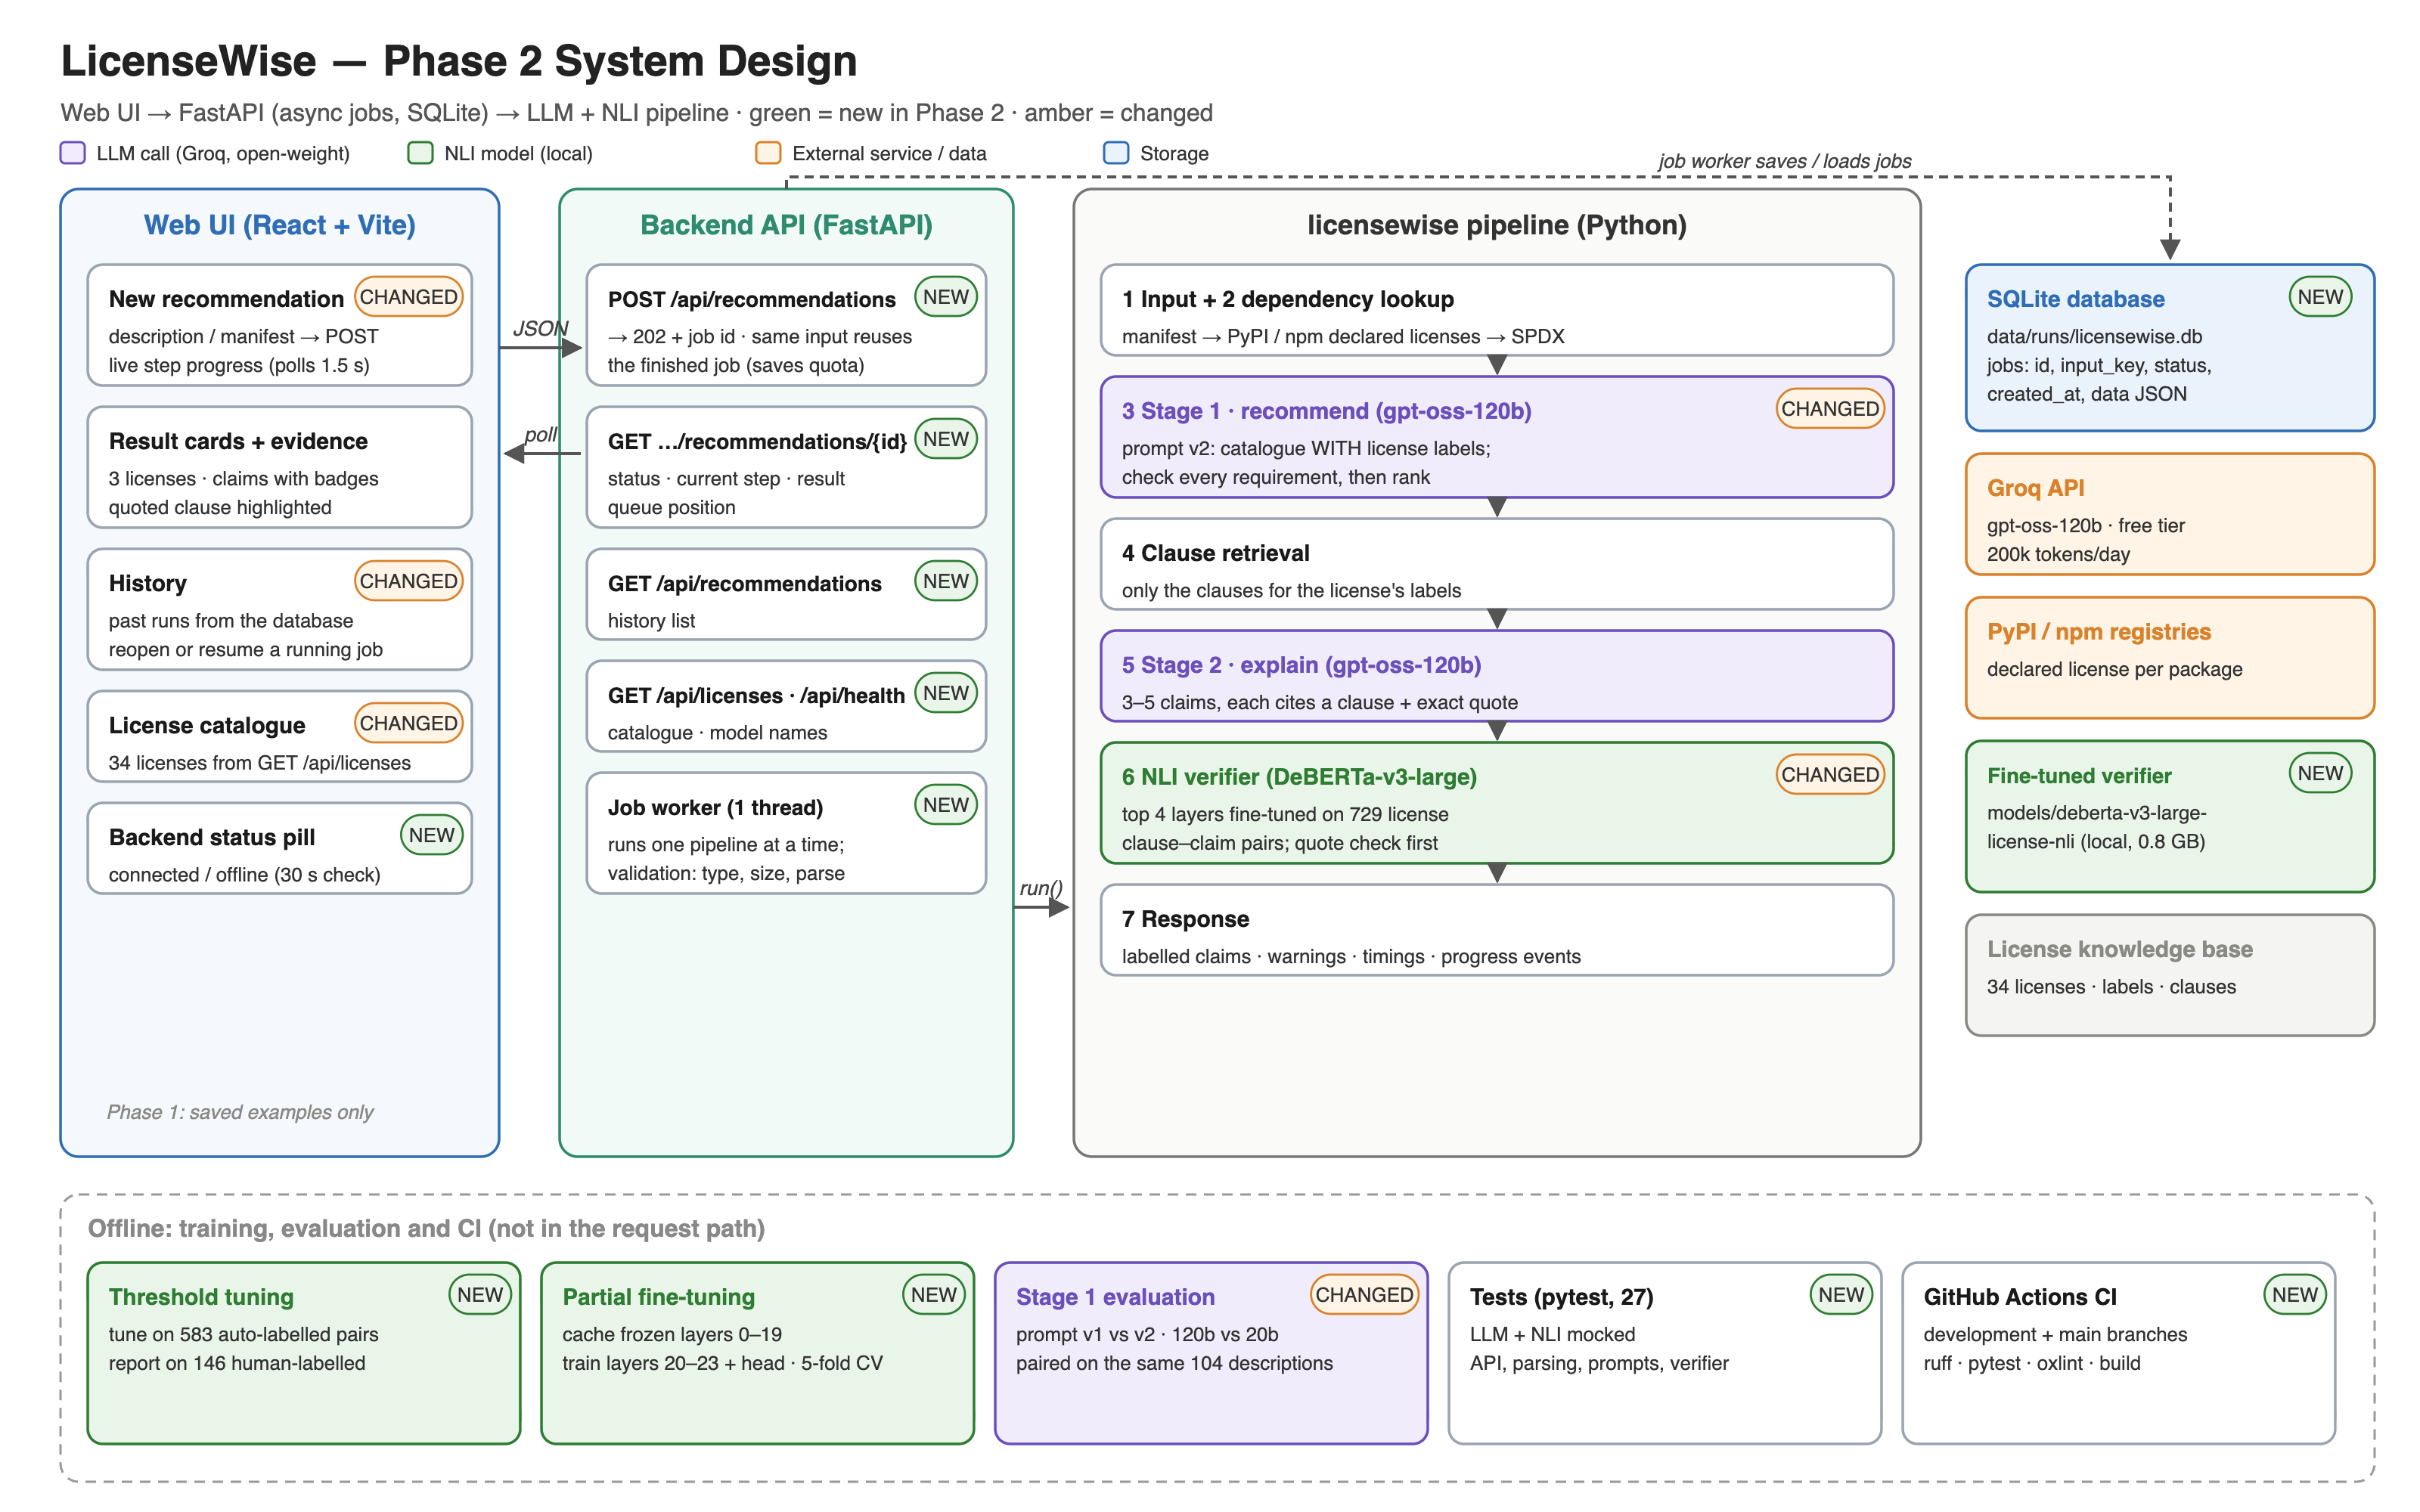
\includegraphics[width=0.94\textwidth]{p2_07_system_design_v2.png}
    \caption{Phase 2 system design. Green tags mark components new in Phase~2 and amber tags components changed since Phase~1. The offline strip holds training, evaluation, and CI, which are not in the request path.}
    \label{fig:arch}
\end{figure*}

\subsection{Implementation}
\label{ss:impl}

Table~\ref{tab:impl} lists the technology stack. The code is in the GitHub repository \texttt{AJFX-01/softwarelincense}. The pipeline is a Python package, \texttt{licensewise}, with one module per step; every LLM call requests output that conforms to a Pydantic JSON schema, and the Stage~1 schema restricts identifiers to the 34 catalogue entries. Input is validated before any LLM call: a description or a manifest is required, descriptions are capped at 4{,}000 characters, and manifests must be \texttt{requirements.txt}, \texttt{pyproject.toml}, or \texttt{package.json}, at most 100\,KB, parse correctly, and list dependencies. Invalid input returns HTTP 422. Rate-limit and missing-key errors are reported in plain language. If a request exceeds the free tier's per-minute token limit (HTTP 413), it is retried once with a smaller output cap.

\begin{table}[tb]
    \caption{Implementation stack.}
    \label{tab:impl}
    \centering
    \footnotesize
    \begin{tabularx}{\columnwidth}{@{}lX@{}}
        \toprule
        \textbf{Layer} & \textbf{Technology} \\
        \midrule
        Front end & React 19, TypeScript, Vite; pages for new recommendation, history, and licenses \\
        Backend & FastAPI + Uvicorn (Python 3.14); 5 endpoints; 1 worker thread \\
        Database & SQLite (Python standard library) \\
        LLM & gpt-oss-120b via Groq, JSON-schema output (Stages 1 and 2) \\
        Verifier & DeBERTa-v3-large NLI, top 4 of 24 layers fine-tuned (PyTorch, Transformers, Apple MPS); runs locally, 0.8\,GB \\
        Data & choosealicense.com, SPDX, Software Heritage, PyPI, npm \\
        Quality & pytest (27 tests), ruff, oxlint, \texttt{tsc} \\
        CI/CD & GitHub Actions; branches \texttt{development} and \texttt{main} \\
        \bottomrule
    \end{tabularx}
\end{table}

\subsection{Database}
\label{ss:db}

Jobs are stored in a single SQLite table, \texttt{jobs(id, input\_key, status, created\_at, data)}, indexed on \texttt{created\_at}. SQLite suits a single-user tool: it needs no server, writes are atomic (a crash cannot leave a half-written record, which happened with the Phase~1 JSON files), and history can be queried by status and time. \texttt{input\_key} is a SHA-256 hash of the model, description, manifest, and verification flag; an identical request reuses the finished result instead of spending LLM quota again. \texttt{data} holds the full nested pipeline result as JSON because its shape is still evolving. On startup, jobs left queued or running by a restart are marked failed with a clear message, and Phase~1 job files are imported once.

\subsection{UI and Backend Integration}
\label{ss:ui}

The UI calls \texttt{GET /api/health} every 30\,s to show a ``backend connected/offline'' indicator; \texttt{POST /api/recommendations} starts a run (or reuses an identical one); \texttt{GET /api/recommendations/\{id\}} reports the live step (dependency lookup, Stage~1, retrieval, explanation, verification); \texttt{GET /api/recommendations} lists history; and \texttt{GET /api/licenses} serves the catalogue with labels and copyleft level. Figure~\ref{fig:ui} shows the user flow: enter a description or manifest, follow the run, read three license cards whose claims carry status badges, and open the cited clause with the quoted words highlighted and the NLI probabilities. Badges combine an icon with a text label, so status is never conveyed by colour alone.

\begin{figure}[tb]
    \centering
    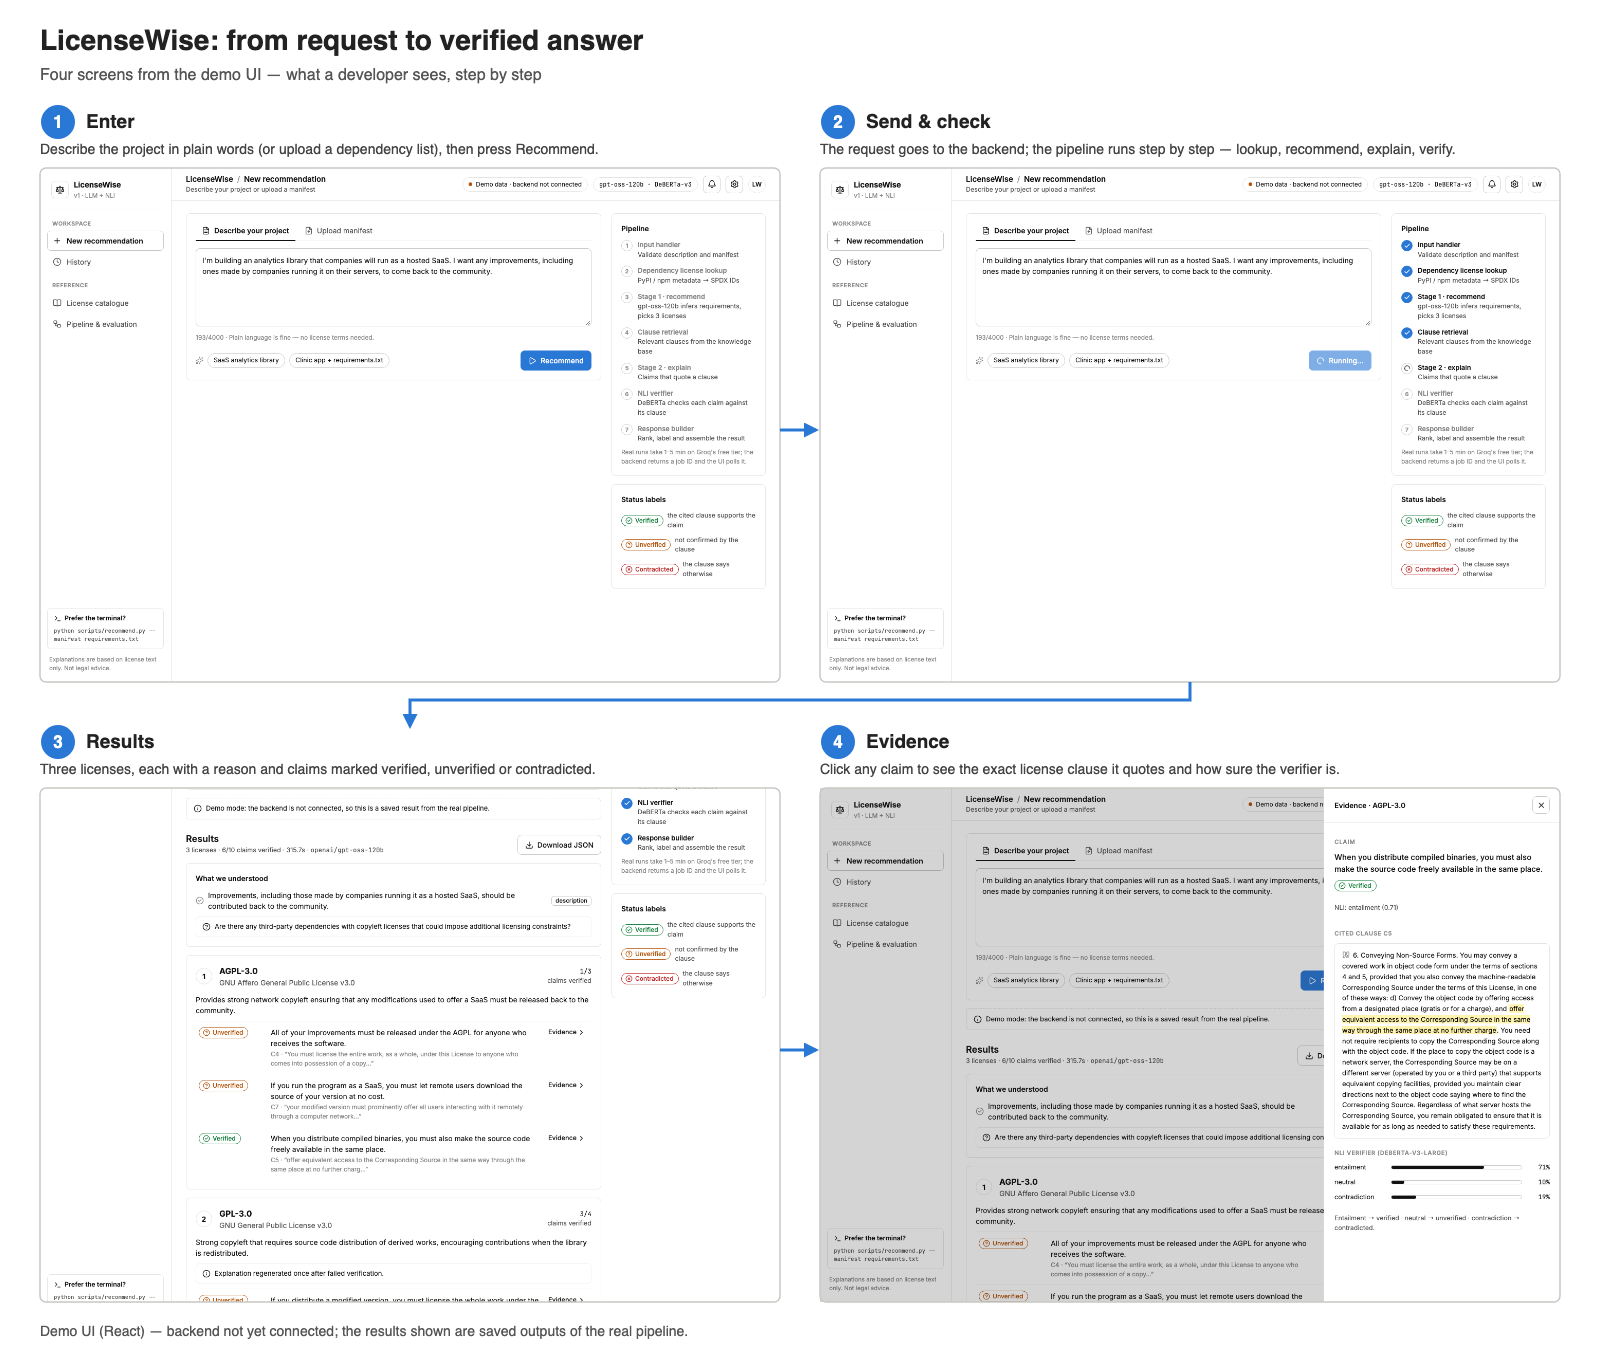
\includegraphics[width=\columnwidth]{22_ui_storyboard.png}
    \caption{User flow: (1) input, (2) live pipeline steps, (3) results with verified/unverified/contradicted claims, (4) evidence with the highlighted clause.}
    \label{fig:ui}
\end{figure}

\subsection{CI/CD and GitHub Integration}
\label{ss:ci}

Figure~\ref{fig:ci} shows the workflow. Work lands on \texttt{development}; \texttt{main} is the stable, demo-ready branch and changes only through a pull request whose checks pass. GitHub Actions runs on every push and pull request to either branch, with two jobs. The \emph{backend} job installs a CI requirements file and runs \texttt{ruff} and \texttt{pytest}. The \emph{ui} job installs dependencies with a frozen lockfile and runs \texttt{oxlint}, the TypeScript type-check, and the Vite build, so the UI that talks to the API is checked on every change. The 27 tests replace the LLM and NLI calls with fakes and use a temporary database, so CI needs no API key or model, installs no PyTorch, and runs the suite in under a second. The tests cover the API contract (202 and polling, reuse, 422/404 errors, persistence across restarts), manifest parsing, license normalisation, the Stage~1 prompt variants and retry logic, and the verifier's quote check. They also found a real defect: the worker pool was created at import time, so the application could not restart within one process; it is now created in the FastAPI lifespan handler.

\begin{figure*}[tb]
    \centering
    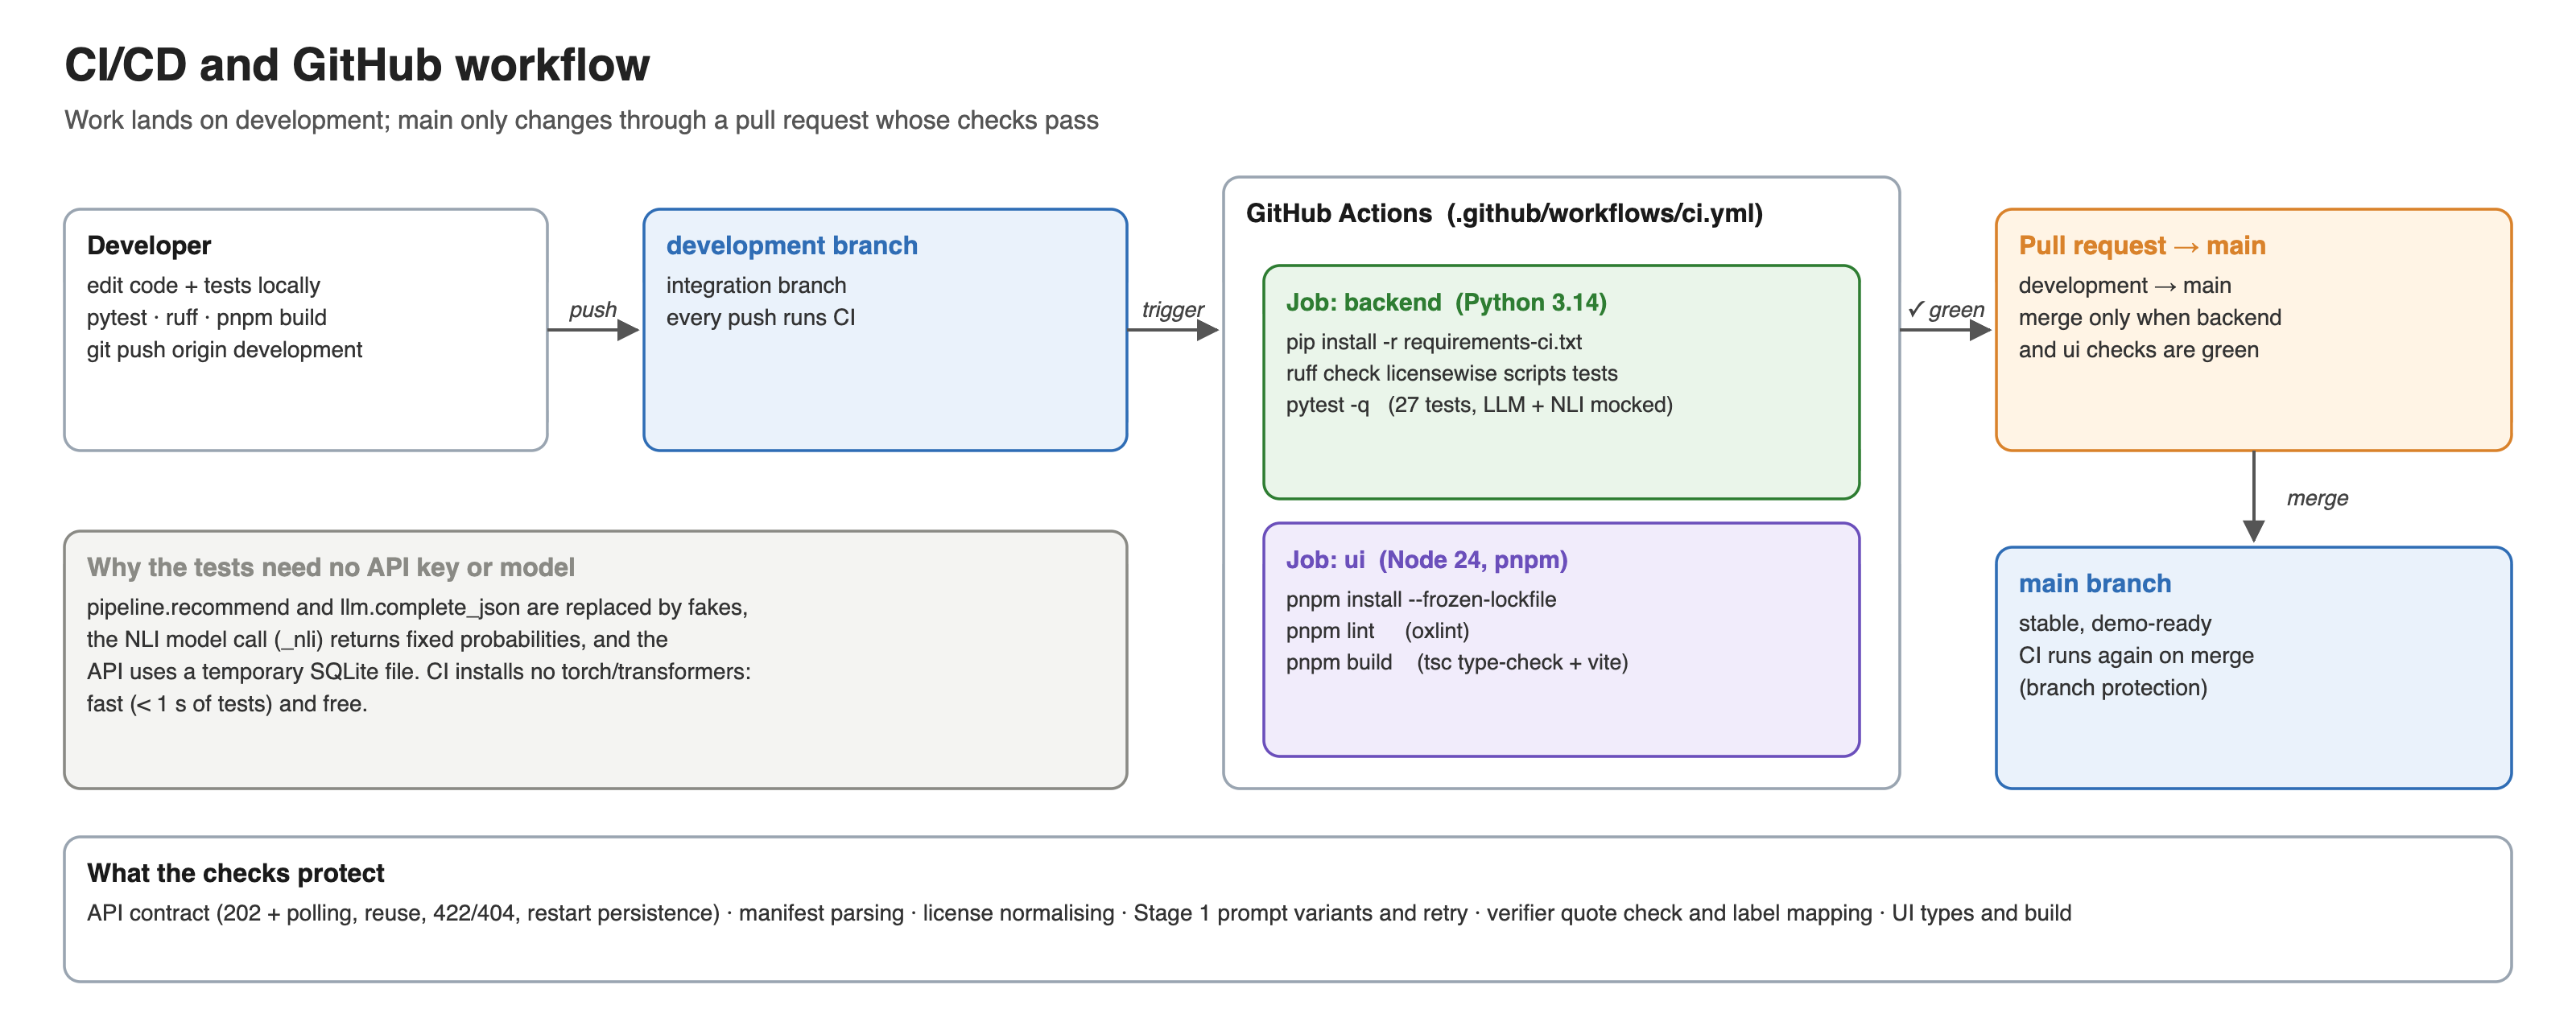
\includegraphics[width=0.85\textwidth]{p2_08_cicd.png}
    \caption{CI/CD workflow: pushes to \texttt{development} trigger the backend and UI jobs; \texttt{main} changes only through a pull request with passing checks.}
    \label{fig:ci}
\end{figure*}

\section{Machine Learning Components}
\label{s:ml}

\subsection{What Changed Since Phase 1}
\label{ss:mlchanges}

\subsubsection{Data}
No new data were labelled. The 729 clause--claim pairs, used only for testing in Phase~1, became training data for the verifier through cross-validation. The training target is the human label where one exists (146 pairs) and the automatic label otherwise, which matches the human labels on 97.9\% of checked pairs. The 104 Stage~1 descriptions are unchanged, so every Stage~1 comparison is \emph{paired} with Phase~1.

\subsubsection{Data transformation}
The verifier is trained with its lower layers frozen. Their output for a pair never changes, so it is computed once for all 729 pairs and cached on disk in half precision (185\,MB); training then runs only the top layers. This is mathematically equivalent to training the full model with those layers frozen. Before training, the cached model reproduced the Phase~1 predictions on 729 of 729 pairs (maximum probability difference 0.0016). Stage~1 received a richer input: each catalogue line now carries the license's permission, condition, and limitation labels (about 1{,}500 extra input tokens).

\subsubsection{Evaluation}
Metrics are unchanged so that Phase~1 and Phase~2 numbers compare directly. For RQ1: Hit@1 (first pick in the answer key), Hit@3 (any of three), Precision@3 (share of the three), and, for each requirement, the share of picks that violate it, grouped by answer-key size. For RQ2: accuracy, macro-F1, and per-class precision and recall on the 146 human-labelled pairs. The key metrics are \emph{verified precision} (entailment precision, the faithfulness requirement, target $\geq 0.90$) and the share of true claims confirmed (entailment recall).

\subsection{Verifier Configurations and Fine-Tuning}
\label{ss:verifiermethod}

We explored four verifier configurations against the Phase~1 baseline, DeBERTa-v3-large with an argmax decision.

\subsubsection{Threshold tuning}
The claim is \emph{verified} if $P(\text{entailment}) \geq t$; otherwise the larger of neutral and contradiction is used. We swept $t$ from 0.05 to 0.95 and chose the best macro-F1 that keeps entailment precision $\geq 0.90$ on the 583 pairs \emph{without} human labels, then reported on the 146 human pairs, which play no part in the choice. The chosen threshold was $t = 0.10$.

\subsubsection{Partial fine-tuning}
The development laptop has 8\,GB of unified memory, and full fine-tuning of the 435M-parameter model needs about 7\,GB for optimiser state alone. We therefore train only the top $K$ of 24 encoder layers plus the pooler and classifier; $K$ is the architectural hyperparameter. Partial fine-tuning keeps the broad NLI pre-training that made the large model the best Phase~1 verifier, which a smaller model would lose. Table~\ref{tab:hparams} lists the settings.

\begin{table}[tb]
    \caption{Verifier fine-tuning setup.}
    \label{tab:hparams}
    \centering
    \footnotesize
    \begin{tabularx}{\columnwidth}{@{}lX@{}}
        \toprule
        \textbf{Choice} & \textbf{Value and reason} \\
        \midrule
        Base model & DeBERTa-v3-large NLI (MNLI, FEVER, ANLI, LingNLI, WANLI)~\cite{laurer2024less} \\
        Trainable layers & $K \in \{2, 4, 8\}$; $K=4$ chosen ($K=2$ under-fits; $K=8$ ran out of memory) \\
        Optimiser & AdamW, learning rate $2\times10^{-5}$, weight decay 0.01, 10\% warm-up, gradient clipping 1.0 \\
        Epochs / batch & 3 / 8, batches of similar-length pairs \\
        Precision & cached frozen outputs in float16; trained layers in float32 \\
        Validation & 5-fold cross-validation grouped by license; out-of-fold predictions \\
        Selection & $K$ chosen on the 583 automatically labelled pairs (accuracy 0.919 for $K=2$, 0.942 for $K=4$) \\
        Final model & retrained on all 729 pairs (about 4 minutes); deployed in the application \\
        \bottomrule
    \end{tabularx}
\end{table}

Folds are grouped by license, so every prediction comes from a model that never saw that license; random splits would place the same clause, with a different claim, in both training and test data. Because all claims come from 16 templates, a model could also learn the templates' wording instead of reading clauses. As a stress test we therefore repeated cross-validation with folds grouped by \emph{label}, so that the claim templates of a held-out label never appear in training; this is the closer estimate for the new wording that Stage~2 produces.

\subsubsection{Engineering for a laptop}
The first attempt, with the whole model loaded and the lower layers frozen, swapped about 13\,GB and finished no epoch in six minutes; caching the frozen layers fixed it. A second slowdown came from the Apple MPS allocator keeping buffers for every batch shape: clearing its cache every 20 steps cut an epoch from 33\,min to 63\,s with an identical loss.

\subsection{Stage 1 Prompt and Model Configurations}
\label{ss:stage1method}

The Phase~1 error analysis showed that the requirements violated most often (trademark, change documentation, network use) are exactly the facts in the license labels, which the Phase~1 catalogue omitted, so the model had to recall them. \emph{Prompt v2} (i) appends each license's labels to its catalogue line, (ii) explains how to read the labels that were misused (e.g., \texttt{trademark-use} under limitations means trademarks are \emph{not} granted), and (iii) asks the model to list the stated requirements, keep only licenses that satisfy all of them, and then rank. To test whether model size matters more than grounding, we also ran the Phase~1 prompt on the smaller gpt-oss-20b.

Groq's free tier allows 200{,}000 tokens per model per day, and one description costs about 4{,}200 tokens with prompt v1 and 6{,}000 with v2, so a full comparison takes several days. We therefore tried \emph{one} new prompt, designed from the Phase~1 error analysis before any new results were seen, and ran all configurations on the same 104 descriptions as Phase~1. Since no prompt was selected on the test set, no separate tuning split was needed, and every difference is a paired comparison.

\section{Results}
\label{s:results}

\subsection{RQ1: Requirement-to-License Mapping}
\label{ss:rq1}

\begin{table}[tb]
    \caption{Stage 1 configurations on the same 104 descriptions.}
    \label{tab:stage1}
    \centering
    \footnotesize
    \begin{tabular}{@{}lrrr@{}}
        \toprule
        \textbf{Configuration} & \textbf{Hit@1} & \textbf{Hit@3} & \textbf{Prec@3} \\
        \midrule
        Prompt v1, gpt-oss-120b (Phase 1) & 0.558 & 0.740 & 0.548 \\
        \textbf{Prompt v2, gpt-oss-120b} & \textbf{0.885} & \textbf{0.942} & \textbf{0.849} \\
        Prompt v1, gpt-oss-20b & 0.548 & 0.692 & 0.519 \\
        \bottomrule
    \end{tabular}
\end{table}

\begin{figure}[tb]
    \centering
    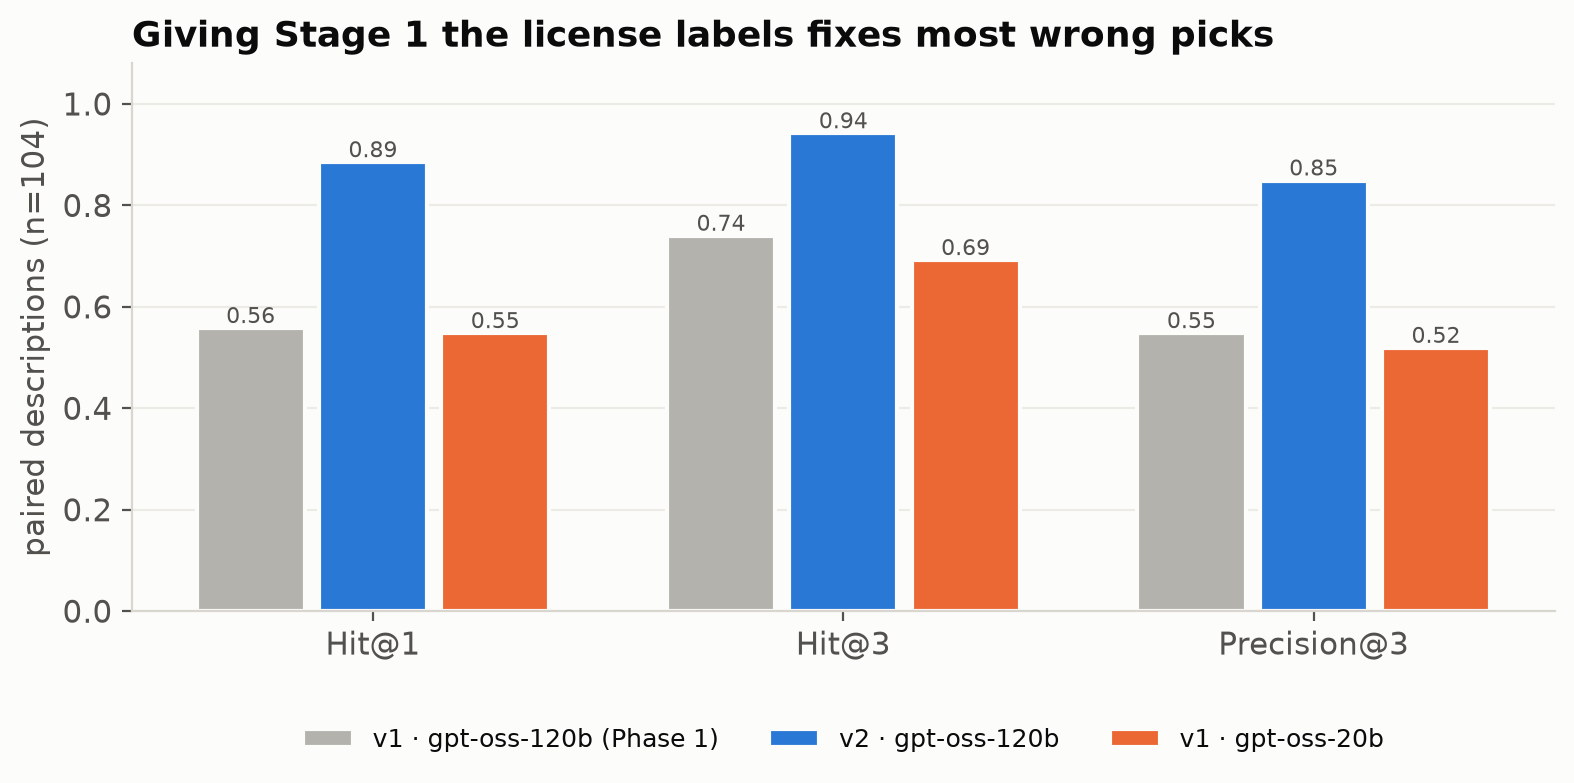
\includegraphics[width=\columnwidth]{p2_05_stage1_configs.png}
    \caption{RQ1: Stage 1 configurations on 104 paired descriptions.}
    \label{fig:stage1}
\end{figure}

Table~\ref{tab:stage1} and Fig.~\ref{fig:stage1} answer the new part of RQ1. Grounding the model in the license labels raised top-pick accuracy from 0.558 to 0.885 and top-3 accuracy from 0.740 to 0.942. The smaller model with the original prompt was slightly worse than the baseline on every metric, so grounding matters far more than model size, and gpt-oss-120b remains the deployed model. The cost is about 40\% more tokens per description, and 6 of 104 requests initially exceeded the free tier's per-minute limit; all succeeded when retried with a smaller output cap.

\begin{table}[tb]
    \caption{Hit@1 / Hit@3 by number of correct licenses (answer-key size).}
    \label{tab:spec}
    \centering
    \footnotesize
    \begin{tabular}{@{}lrcc@{}}
        \toprule
        \textbf{Correct licenses} & \textbf{n} & \textbf{v1 (Phase 1)} & \textbf{v2 (Phase 2)} \\
        \midrule
        1--3 (hardest) & 47 & 0.40 / 0.60 & 0.77 / 0.87 \\
        4--10 & 35 & 0.54 / 0.77 & 0.97 / 1.00 \\
        $>$10 (easiest) & 22 & 0.91 / 1.00 & 1.00 / 1.00 \\
        \bottomrule
    \end{tabular}
\end{table}

Table~\ref{tab:spec} shows the effect of specificity. Prompt v2 is near-perfect when four or more licenses fit, and it nearly doubles top-pick accuracy on the hardest requests (0.40 to 0.77), but those requests remain the weakest group: when only one to three licenses fit, the top three miss every correct license for 13\% of descriptions.

\begin{figure}[tb]
    \centering
    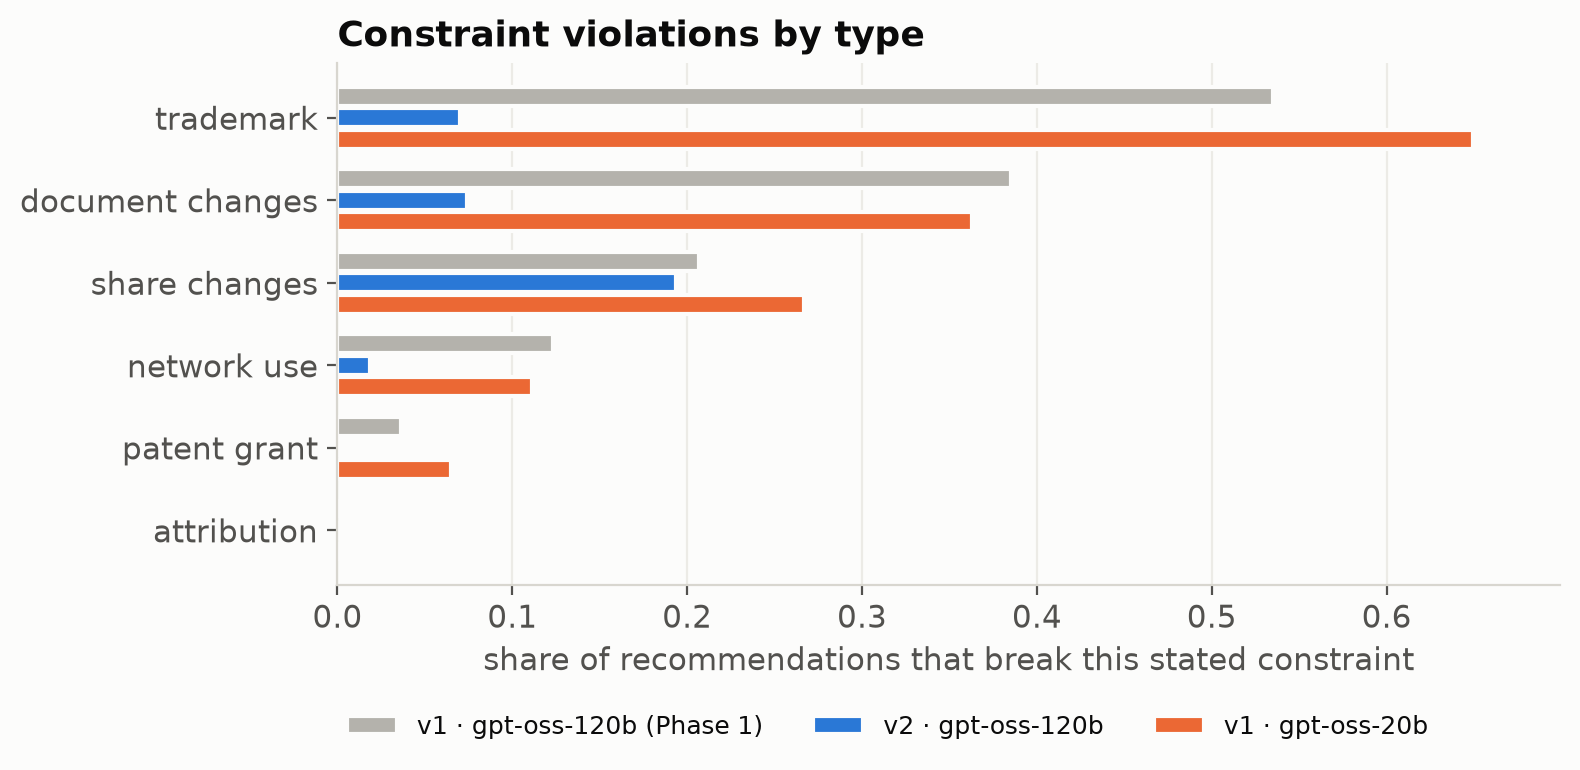
\includegraphics[width=\columnwidth]{p2_06_stage1_violations.png}
    \caption{RQ1: share of recommendations that break each stated requirement.}
    \label{fig:viol}
\end{figure}

Fig.~\ref{fig:viol} shows why. The labels fixed the requirements they state directly: picks that break trademark protection fell from 0.54 to 0.07, change documentation from 0.39 to 0.07, network use from 0.12 to 0.02, and patent grant from 0.04 to 0. The copyleft level barely moved (0.21 to 0.19). Of the 14 descriptions with a copyleft miss, 12 ask for \emph{weak} copyleft (LGPL- or MPL-style, at file or library level), for which only two to four licenses fit; the model mostly falls back to permissive licenses such as Apache-2.0. The v2 prompt explained the trademark, change-documentation, and network labels but not the file- and library-level copyleft labels. We did not patch the prompt after seeing these results, because that would tune it on the test set.

\subsection{RQ2: Claim Verification}
\label{ss:rq2}

\begin{table}[tb]
    \caption{Verifier configurations on 146 human-labelled pairs. Ver.\ prec.\ = verified (entailment) precision; Conf.\ = share of true claims confirmed (entailment recall).}
    \label{tab:verifier}
    \centering
    \footnotesize
    \begin{tabular}{@{}lccc@{}}
        \toprule
        \textbf{Configuration} & \textbf{Acc.} & \textbf{Ver.\ prec.} & \textbf{Conf.} \\
        \midrule
        RoBERTa-large-MNLI (Phase 1) & 0.733 & 0.900 & 0.551 \\
        DeBERTa, argmax (Phase 1) & 0.815 & 0.944 & 0.694 \\
        DeBERTa, threshold $t=0.10$ & 0.829 & 0.925 & 0.755 \\
        Fine-tuned, $K=2$ & 0.897 & 0.936 & 0.898 \\
        \textbf{Fine-tuned, $K=4$} & \textbf{0.925} & \textbf{0.978} & \textbf{0.918} \\
        \midrule
        $K=4$, unseen claim wording & 0.911 & 0.933 & 0.857 \\
        \bottomrule
    \end{tabular}
\end{table}

Table~\ref{tab:verifier} compares the configurations. Threshold tuning alone confirmed 9\% more true claims at a cost of two points of precision. Fine-tuning the top four layers improved every metric: accuracy rose from 0.815 to 0.925 and macro-F1 from 0.816 to 0.925, true claims confirmed rose from 69\% to 92\%, and verified precision rose from 0.944 to 0.978. Training more layers helped ($K=2 \rightarrow 4$) until memory ran out at $K=8$. Because the fine-tuned model's verified precision is already well above the target, it uses the plain argmax rule; the threshold was tuned for the base model.

\begin{figure}[tb]
    \centering
    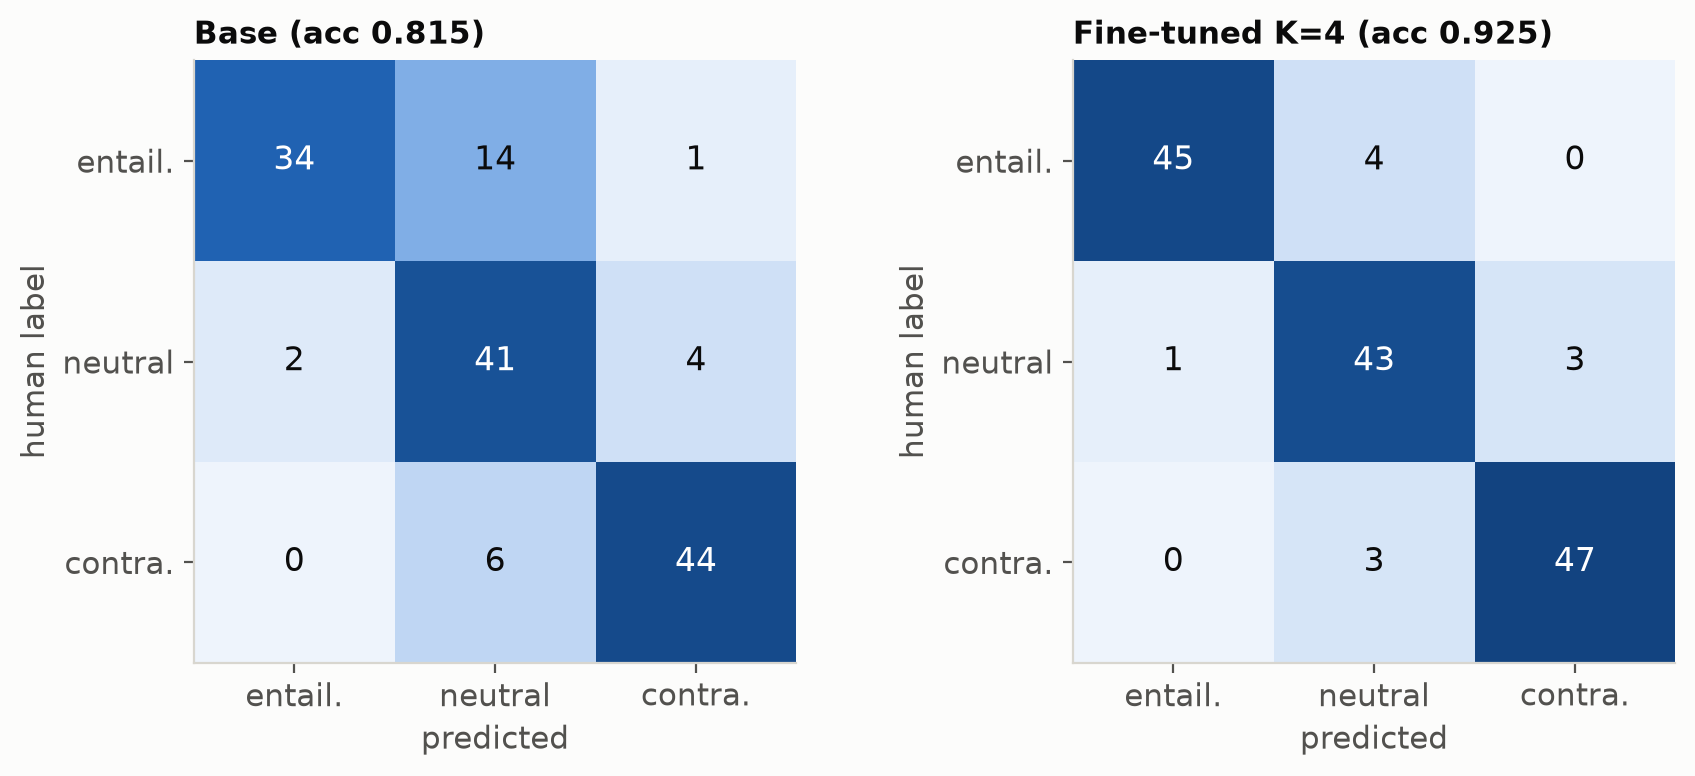
\includegraphics[width=\columnwidth]{p2_03_confusion_base_vs_finetuned.png}
    \caption{RQ2: confusion matrices on 146 human-labelled pairs, base DeBERTa (left) and fine-tuned $K=4$ (right). Rows are human labels.}
    \label{fig:cm}
\end{figure}

Fig.~\ref{fig:cm} shows where the gain comes from. Errors fell from 27 to 11 of 146. True claims judged neutral (shown as \emph{unverified}) fell from 14 to 4. Only one neutral claim was marked verified, and no contradiction was marked verified, so the cautious behaviour that suits licensing is preserved.

\subsubsection{Does the verifier memorise claim wording?}
With folds grouped by label, so that the test claims' wording is never seen in training, accuracy is 0.911, verified precision 0.933, and 86\% of true claims are confirmed (Table~\ref{tab:verifier}, last row). Most of the gain therefore generalises, and the faithfulness target ($\geq 0.90$) is met in both settings. Fig.~\ref{fig:mem} shows the gains per label. Patent-use claims go from 0.41 to 0.94 and trademark claims from 0.55 to 1.00 even with unseen wording. Commercial-use claims, however, rise from 0.21 to 1.00 when the wording was seen but to only 0.33 when it was not: that part of the gain is memorised. With unseen wording, one contradiction was also marked verified (base model: none). We report the unseen-wording score as the honest estimate for new claims.

\begin{figure}[tb]
    \centering
    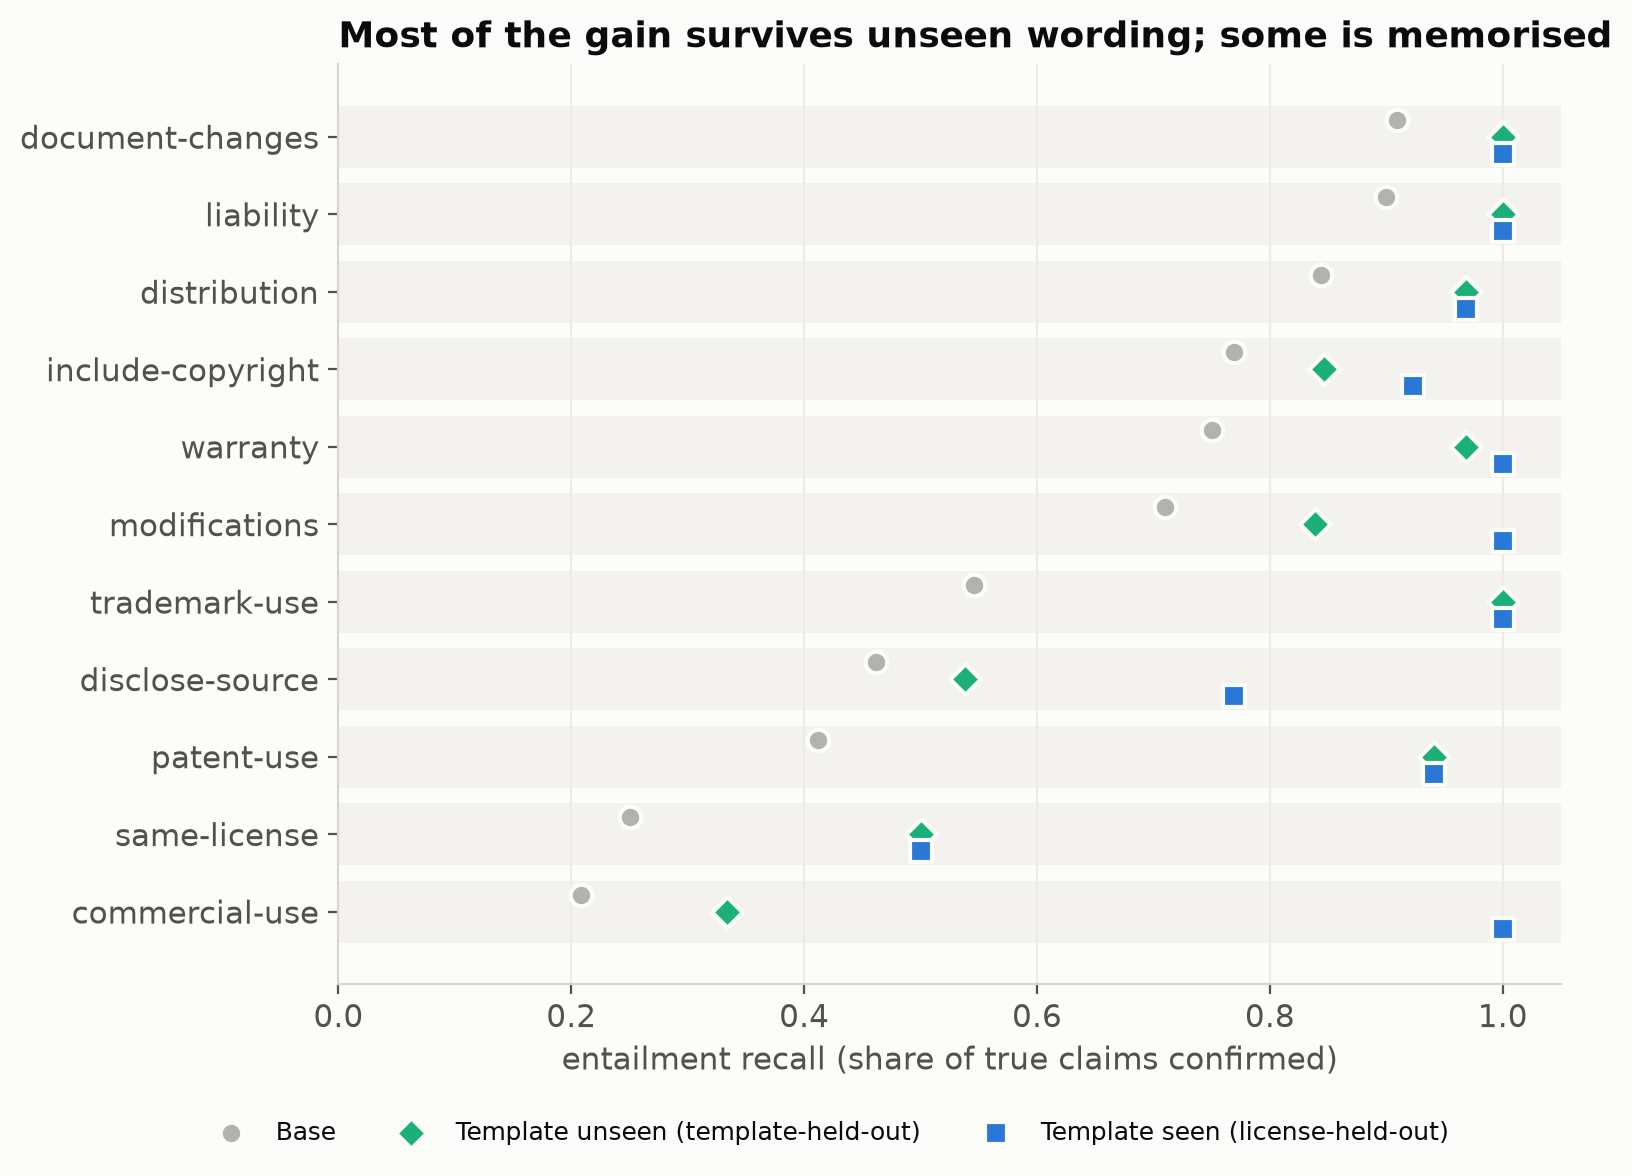
\includegraphics[width=\columnwidth]{p2_04_template_memorisation.png}
    \caption{RQ2: share of true claims confirmed per label for the base model and the fine-tuned model, with claim wording seen and unseen in training.}
    \label{fig:mem}
\end{figure}

\subsection{RQ3: Explanation Faithfulness}
\label{ss:rq3}

In Phase~1, all 19 quotes in two end-to-end runs were found verbatim in their cited clauses, and 58\% of claims were verified. In Phase~2 we re-verified the 37 real Stage~2 claims with a verbatim quote from all saved runs, without new LLM calls, using both verifiers. With the base model, 24 claims were verified, 11 unverified, and 2 contradicted; with the fine-tuned model, 32 were verified, 4 unverified, and 1 contradicted. All eight changed claims read as correct against their clauses, including the Phase~1 false contradiction on AGPL-3.0 section~6. Compared with an unverified (LLM-only) baseline, which would show all 37 claims as equally trustworthy, verification now flags 5 claims for the user to check against the clause instead of 13. This is a preview: these claims are not human-labelled, and the systematic RQ3 study remains future work (Section~\ref{s:future}).

\subsection{Evaluation Against the Requirements}
\label{ss:reqs}

\begin{table}[tb]
    \caption{Phase 2 status against the project requirements.}
    \label{tab:reqs}
    \centering
    \footnotesize
    \begin{tabularx}{\columnwidth}{@{}lX@{}}
        \toprule
        \textbf{Requirement} & \textbf{Phase 2 status} \\
        \midrule
        FR1/FR2 description and/or manifest & Met, in UI and API, validated \\
        FR4 recommend 3 fitting licenses & Met: Hit@3 0.94 (Phase 1: 0.74) \\
        FR5 explain with cited clauses & Met: every claim quotes a clause \\
        FR6 verify each claim & Met: fine-tuned verifier \\
        FR11 operational warnings & Met: rate limit, missing key, invalid input \\
        NFR faithfulness (ver.\ prec.\ $\geq 0.90$) & Met: 0.978; 0.933 on unseen wording \\
        NFR latency ($<$ 5 min, free tier) & Met: about 30--35\,s in our runs; longer when queued or rate-limited \\
        NFR cost & Met: free API tier and a local verifier \\
        NFR security and robustness & Met: type, size, and parse checks before any LLM call; input never executed \\
        NFR reproducibility & Met: pinned dependencies, seeds, tests, CI, decision log \\
        \bottomrule
    \end{tabularx}
\end{table}

Table~\ref{tab:reqs} compares the system with the requirements set in Phase~1. All prioritised functional requirements and the faithfulness requirement are met. Dependency conflicts (FR7) are flagged from declared licenses only; a full compatibility check against the OSADL matrix remains future work.

\section{Discussion}
\label{s:discussion}

\subsection{Key Findings}

\subsubsection{Grounding beats model size}
Giving the LLM the license facts it previously had to recall raised Hit@1 from 0.56 to 0.885, whereas a smaller model with the old prompt did slightly worse than the baseline. The remaining errors concentrate on the one requirement the prompt did not explain (weak copyleft). The LLM is good at turning informal intent into requirements, but license facts should be supplied to it, not recalled from its training.

\subsubsection{Domain adaptation fixes the verifier's blind spot}
In Phase~1 the verifier missed claims whose wording differed from the license text (``sell'' versus ``commercial use''). Fine-tuning four layers on 729 pairs raised the share of true claims confirmed from 69\% to 92\% while verified precision stayed above 0.9, and most of the gain holds for wording not seen in training.

\subsubsection{Fine-tuning a large verifier is feasible on a laptop}
Caching the frozen layers and managing accelerator memory turned an out-of-memory job into a four-minute training run on an 8\,GB machine.

\subsubsection{Expert-free evaluation works}
Answer keys computed from curated labels, test inputs written by one model and checked by another, and a small human-checked label set gave paired comparisons whose effects are large relative to the measured label noise.

\subsection{Impact}
A developer now receives a project-specific license recommendation with explanations they can check clause by clause, instead of a generic quiz or an unverifiable chatbot answer. The whole system runs on a free API tier and a laptop, which matters for students and small teams, the users least able to pay for legal advice. The tool is not legal advice; it is a faster and transparent first step.

\subsection{Strengths and Weaknesses}

\subsubsection{Strengths}
A correct license is in the top three for 94\% of descriptions and the top pick is right for 88.5\%. A \emph{verified} label is reliable (precision 0.98, 0.93 on unseen wording). Every claim is traceable to an exact clause, and the system is tested, continuously integrated, and reproducible, with each design decision and its reason recorded in a project log.

\subsubsection{Weaknesses}
Weak-copyleft requests still often receive permissive picks. Part of the verifier's gain is memorised template wording, and with unseen wording it marked one false claim as verified. Prompt v2 costs about 40\% more tokens, and the free-tier quota limits how many configurations can be compared.

\subsection{Threats to Validity}
\emph{Construct validity:} the ground truth is the choosealicense.com label set, a simplification of legal text with some debatable labels (e.g., EPL is labelled \emph{same license} although often described as weak copyleft), and the six requirements were chosen by us from the labels. \emph{Internal validity:} test descriptions are written and validated by LLMs and may be cleaner than real requests; weak copyleft is under-represented because the round-trip filter rejected more of those descriptions. Prompt v2 was designed after seeing Phase~1 errors on the same 104 descriptions; it was fixed before any v2 result was seen and not revised afterwards, but some optimism towards this set cannot be excluded. \emph{External validity:} the catalogue holds only OSI-approved software licenses, the verifier is English-only (CeCILL-2.1 cannot be verified), and results are for one LLM family. \emph{Reliability:} LLM outputs are non-deterministic and runs were not repeated to measure variance; the RQ3 comparison is small and not human-labelled.

\section{Future Work}
\label{s:future}

\begin{itemize}
    \item \textbf{Weak copyleft:} explain the file- and library-level copyleft labels in the prompt, and re-test on \emph{new} descriptions to avoid tuning on the current set.
    \item \textbf{Verifier generalisation:} paraphrase each claim template several times before fine-tuning to reduce memorisation, and human-label real Stage~2 claims to complete RQ3 with a verified-versus-unverified study and blind agreement.
    \item \textbf{Deterministic checks:} add a rule engine over the labels and the OSADL compatibility matrix~\cite{osadl} to check picks and dependency conflicts after the LLM.
    \item \textbf{Cost and stability:} a compact label-only catalogue to stay under per-request limits, and self-consistency voting for Stage~1.
    \item \textbf{Users and scope:} a user study with developers on clarity and trust, non-OSI and custom licenses, and deployment behind authentication.
\end{itemize}

\section{Conclusion}
\label{s:conclusion}

Phase~2 turned \sys{} from a prototype into a connected application, with a FastAPI backend, SQLite history, a React UI, tests, and CI/CD on a two-branch workflow, and it addressed both weaknesses found in Phase~1. Grounding the recommender in license labels raised top-pick accuracy from 0.56 to 0.885, and fine-tuning the verifier raised its accuracy from 0.815 to 0.925 with verified precision of 0.98. Across both phases, the project shows that an LLM paired with an independent, domain-adapted verifier can give project-specific license advice that a developer can check clause by clause, and that such a system can be evaluated rigorously without a legal expert.

\section*{Individual Contributions}
\todo{Opeyemi Ajegbomogun: ...}\\
\todo{Okemawo Obadofin: ...}


\bibliographystyle{IEEEtran}
\bibliography{references}

\end{document}
